\documentclass[tikz,border=4pt]{standalone}
\usepackage{ctex}
\usepackage{amsmath}
\usepackage{pgfplots}
\pgfplotsset{compat=1.18}

% p10-01c: 抛物线的对称轴与顶点（y = x^2 - 2x - 3，对称轴x=1，顶点(1,-4)）
\begin{document}
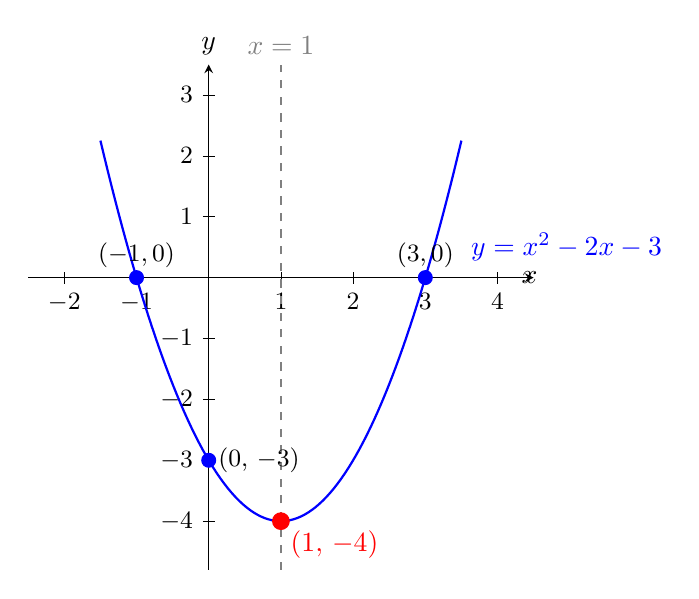
\begin{tikzpicture}
\begin{axis}[
  width=8cm, height=8cm,
  axis lines=center,
  xlabel={$x$}, ylabel={$y$},
  every axis x label/.style={at={(axis cs:4.2,0)}, anchor=west},
  every axis y label/.style={at={(axis cs:0,3.5)}, anchor=south},
  xmin=-2.5, xmax=4.5,
  ymin=-4.8, ymax=3.5,
  xtick={-2,-1,1,2,3,4},
  ytick={-4,-3,-2,-1,1,2,3},
  tick style={color=black},
  ticklabel style={font=\small},
  clip=false,
]
  % y = x^2 - 2x - 3
  \addplot[blue, thick, domain=-1.5:3.5, samples=100] {x^2 - 2*x - 3};
  \node[right, blue] at (axis cs:3.5, 0.5) {$y=x^2-2x-3$};

  % 对称轴 x=1（虚线）
  \draw[gray, dashed, thick] (axis cs:1,-4.8) -- (axis cs:1,3.5);
  \node[above, gray] at (axis cs:1,3.5) {$x=1$};

  % 顶点 (1,-4)
  \addplot[only marks, mark=*, mark size=3pt, red] coordinates {(1,-4)};
  \node[below right, red] at (axis cs:1,-4) {$(1,\,-4)$};

  % 零点标注 (-1,0) 和 (3,0)
  \addplot[only marks, mark=*, mark size=2.5pt, blue] coordinates {(-1,0) (3,0)};
  \node[above] at (axis cs:-1,0) {\small$(-1,0)$};
  \node[above] at (axis cs:3,0) {\small$(3,0)$};

  % 纵截距 (0,-3)
  \addplot[only marks, mark=*, mark size=2.5pt, blue] coordinates {(0,-3)};
  \node[right] at (axis cs:0,-3) {\small$(0,\,-3)$};
\end{axis}
\end{tikzpicture}
\end{document}
